
\documentclass[../main.tex]{subfiles}
\hbadness=1000000
\vbadness=1000000

\begin{document}
% Algunas notas sobre referencias que debo usar: 
% \begin{itemize}
%     \item Para el working point \citep{cabral_role_2011}
%     \item Sobre la velocidad \citep{lemarechal_brain_2022, cabrera-alvarez_modeling_2023}
% \end{itemize}
\section{Methods}
\subsection{Resting-state spiking neural network model}
We built a spiking neural network with 22 regions of interest (ROIs) or nodes reproducing the cingulum bundle of the brain, one of the most prominent white matter structures interconnecting frontal, parietal, and temporal lobes \citep{bubb_cingulum_2018}.
Each region was modelled as a balanced fully-connected network with 80 excitatory and 20 inhibitory neurons, whose set of parameters have been tuned to exhibit alpha oscillations.
The dynamics of the membrane potential of each neuron was described by the adaptive exponential integrate-and-fire (\textit{aeif}) model \citep{naud_firing_2008}, while the dynamics of the synapses was described by the alpha function (equation \eqref{eq:alpha-syn}).
Both dynamics were implemented together in the \textit{aeif\_cond\_alpha\_multisynapse} class in the NEST environment package \citep{eppler2009pynest,gewaltig2007nest}.
% The dynamics of each individual region was designed to exhibit alpha oscillations. 
When the regions are interconnected, the oscillatory dynamics are enhanced, resulting in an oscillation frequency of approximately 10 Hz.
% The detailed procedure to achieve it will explain an discussed in subsequent sections.

Mathematically, the dynamics of the neuron $i$ in the population $k$ was described as follows:
\begin{equation}
    \begin{aligned}
    C_{i}\displaystyle\frac{dv^k_i}{dt} &= -g_{\text{L},i}(v^k_i-E_{\text{L},i})+g_{\text{L},i}\Delta_{T,i} \exp \Bigg( \displaystyle\frac{v_i^k-v_{\text{th},i}}{\Delta_{T,i}} \Bigg) \\ 
    & \quad-w^k_i+I^k_i+I^k_{\text{noise},i}-I^k_{\text{syn},i} + I^k_{\text{ext},i},\\
    \tau_{w,i}\displaystyle\frac{dw^k_i}{dt} &= a_i(v^k_i-E_{\text{L},i})-w^k_i,\\
    \text{if } v^k_i & > v_\text{vpeak} 
    \begin{cases}
      v^k_i & \rightarrow v_{\text{reset},i}\\
      w^k_i & \rightarrow w^k_{\text{reset},i} = w^k_i+b_i
    \end{cases},
    \end{aligned}
    \label{eq:snm_aeif}
\end{equation}
where $I_i^k$ is an external bias current.
$I_{noise,i}^{k}$ is a current generated by a Poissonian spike train with a rate $\lambda$ of 2400 Hz that accounted for the activity received from neurons that were not included in the population.
$I_{syn,i}^{k}$ is the sum of all synaptic currents, and $I_{ext,i}^{k}$ is the current produced by an external sinusoidal stimulation.
Parameters without superindex $k$ mean that their values only depend on whether the neuron is excitatory ($i \in [1,80]$) or inhibitory ($i \in [81,100]$).
The values of the whole set of parameters and their description can be found in Table \ref{tab:snmparams}.
These values were selected to replicate the somatic dynamics of the regular spiking pattern of pyramidal cells and the fast-spiking pattern of interneurons in the cortex for the excitatory and inhibitory neurons in the model, respectively \citep{naud_firing_2008}.

The synaptic current $I^k_{\text{syn},i}$ was expressed as the sum of the synapses within each population $I^k_{\text{intra},i}$ (intra-connectivity)  and the synapses between different populations $I^k_{\text{inter},i}$ (inter-connectivity).
While intra-synapses could be both fast excitatory (AMPA) and fast inhibitory (GABA$_\text{A}$), external long-range synaptic projections were assumed only fast excitatory (AMPA):
% \clearpage
\begin{equation}    
    \begin{aligned}
    % I^k_{\text{syn},i} & = I^k_{\text{intra},i} + I^k_{\text{inter},j},\\
    I^k_{\text{intra},i} & = \displaystyle\sum_{j=1}^{n_e}A^{kk}_{ij}g^{kk}_{ij,\text{AMPA}}(t-\delta^{kk}_{ij})(v^k_i-E_\text{AMPA}) \\
    & \quad + \displaystyle\sum_{j=n_e + 1}^{n_e+n_i}B^{kk}_{ij}g^{kk}_{ij,\text{GABA}}(t-\delta^{kk}_{ij})(v^k_i-E_\text{GABA}), \\
    I^k_{\text{inter,i}} & = \omega
    \displaystyle\sum_{\substack{k'=1\\ k'\neq k}}^{N}
\displaystyle\sum_{j=1}^{n_e}A^{kk'}_{ij}g^{kk'}_{ij\text{AMPA}}(t-\delta^{kk'}_{ij})(v^k_i-E_\text{AMPA}),\\
\end{aligned}
\end{equation}
and the conductances are described by the alpha function:
\begin{equation}
\begin{aligned}
    g^{kk'}_{ij,\text{syn}}(t) & = \bar{g}^{kk'}_{ij,\text{syn}}\bigg(\frac{t-t^{k'*}_j}{\tau_\text{syn}}\bigg)
    \exp\bigg(\displaystyle\frac{t-t^{k'*}_j-\tau_\text{syn}}{\tau_\text{syn}} \bigg),
    \end{aligned}
    \label{eq:snn_syncurrent}
\end{equation}
\noindent where $A$ and $B$ are the connectivity matrices for excitatory and inhibitory projections, $\delta$ is the matrix representing the delays in the synaptic connections, $\omega$ is the coupling factor, $\overline{g}_{ij,\text{syn}}^{kk'}$ is the maximum strength of the synapse between presynaptic neuron $j$ from population $k'$ and postsynaptic neuron $i$ from population $k$, and $t_j^{k'*}$ is the time when the presynaptic neuron $j$ in population $k'$ spiked.
The model is driven by the data extracted from subjects.
These data are the interregional weighted connectivity matrix $A^{kk'}$, given by the normalized \textit{tract density matrix}, and the interregional delay matrix $\delta^{kk'}$, obtained by the \textit{tract length matrix} $l^{kk'}$ using the relation $\delta^{kk'} = l^{kk'}/v_{prop}$, where $v_{prop}$ is the propagation velocity and is set at 15 mm/ms \citep{cabrera-alvarez_modeling_2023}, which is in the physiologically realistic range between 5 and 20 m/s \citep{ghosh2008noise,cabral_role_2011}.
\begin{table}[htbp]
    \caption{Spiking neural network model parameters.
    In order to introduce heterogeneity into the model, a jitter has been applied to the parameters of all neurons.}
    \label{tab:snmparams}
    \def\arraystretch{1.2}%  1 is the default, change whatever
    \begin{tabularx}{\textwidth}{|l|c|c|c|X|}
        \hline 
        \textbf{Parameter} & \multicolumn{2}{c|}{\textbf{Value}} & 
        \textbf{Unit} &     \textbf{Description} \\ 
        \cline{2-3}
        & \textbf{exc} & \textbf{inh} &  & \\ 
        \hline
        $C$ & 104 & 59 &  pF & Capacity of the membrane \\ 
        \hline
        $v_\text{reset}$ & -53.0 & -54.0 & mV & Reset value for $v_m$ after a spike \\
        \hline
        $E_\text{L}$ & -65.0 & -62.0 & mV & Leak reversal potential \\
        \hline
        $g_\text{L}$ & 4.3 & 2.9 & nS & Leak conductance \\
        \hline  
        $a$ & -0.8 & 1.8 & ns & Subthreshold adaptation \\
        \hline 
        $b$ & 65.0 & 61.0 & pA & Spike-triggered adaptation \\
        \hline 
        $\Delta T$ & 0.8 & 3.0 & mV & Slope factor\\
        \hline 
        $\tau_w$ & 88.0 & 16.0 & ms & Adaptation time constant \\
        \hline 
        $v_\text{th}$ & -52.0 & -42.0 & mV & Spike initiation threshold\\
        \hline 
        $v_\text{vpeak}$ & \multicolumn{2}{c|}{0.0} & mV & Spike detection threshold\\
        \hline
        $t_\text{ref}$ & \multicolumn{2}{c|}{2.0} & ms & Duration of the refractory period \\
        \hline 
        $I$ & \multicolumn{2}{c|}{variable} & pA & Constant external input current \\
        \hline
        $\bar{g}_\text{AMPA}$ & \multicolumn{2}{c|}{variable} & nS & Maximum conductance of the excitatory synapses \\
        \hline
        $\bar{g}_\text{GABA}$ & \multicolumn{2}{c|}{variable} & nS & Maximum conductance of the inhibitory synapses \\
        \hline
        $\bar{g}_\text{noise}$ & \multicolumn{2}{c|}{variable} & nS & Maximum conductance of background activity synapses (AMPA) \\
        \hline
        $\lambda $ & \multicolumn{2}{c|}{2400} & Hz & Rate of the Poissonian spike train \\
        \hline
        $E_\text{AMPA}$ & \multicolumn{2}{c|}{0.0} & mV & AMPA Excitatory reversal potential \\
        \hline 
        $E_\text{GABA}$ & \multicolumn{2}{c|}{-85.0} & mV & GABA Inhibitory  reversal potential \\
        \hline 
        $\tau_\text{syn,AMPA}$ & \multicolumn{2}{c|}{3.0} & ms & Rise time of AMPA excitatory synaptic conductance \\
        \hline 
        $\tau_\text{syn,GABA}$ & \multicolumn{2}{c|}{3.2} &  ms & Rise time of GABA inhibitory synaptic conductance \\
        \hline 
        $\delta^{kk}$ & \multicolumn{2}{c|}{1.0} & ms & Intra-synaptic delay due to axon length \\
        \hline
        $\delta^{kk'}$ & \multicolumn{2}{c|}{range} & ms & Inter-synaptic ($k\neq k'$) delay due to axon length \\
        \hline
    \end{tabularx}
\end{table}
The output of the network model is a set of 22 time series, representing the local field potential (LFP) of each region.
The LFP was computed as the sum of the absolute value of all synaptic currents of the excitatory neurons in that node \citep{mazzoni_encoding_2008,sancristobal_role_2014,negahbani_neuroimage_2018}:
\begin{equation}
    \text{LFP}^k = \displaystyle\sum_{i=1}^{n_e}|I^k_{\text{AMPA},i} | + |I^k_{\text{GABA},i}|.
    \label{eq:lfp}
\end{equation}
\begin{figure}[htpb]
    \centering
    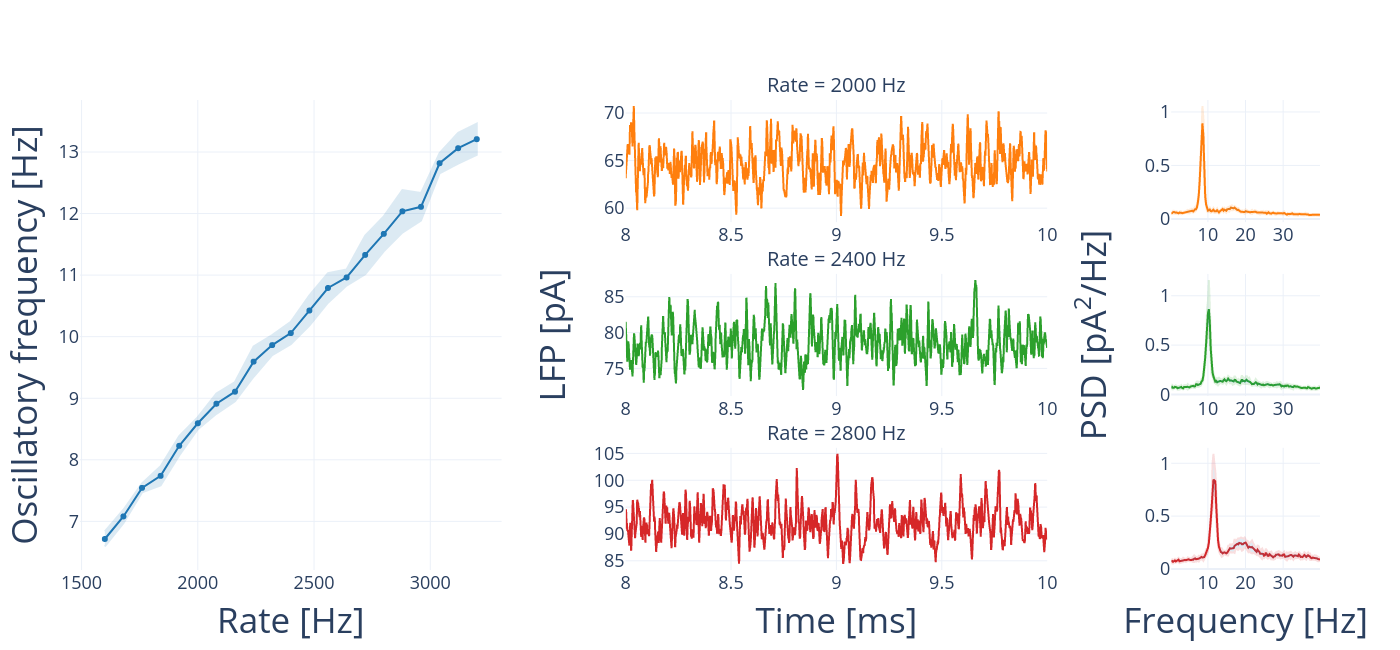
\includegraphics[width=\textwidth]{chapter3/figures/single-node-dynamics.png}
    \caption{\textbf{Single node dynamics}.
    Left panel represents the frequency-current curve, where to control the intensity of the incoming current we used the rate of the Poissonian spike train that every neuron receives.
    Center and left panels show different LFPs for different values of the rate and their power spectral densities, respectively.
    The PSDs are the mean of 10 realizations and shadowed area represent the standard deviation.}
    \label{fig:single-node}
\end{figure}

Figure \ref{fig:single-node} shows the current-frequency curve of a single node and three different time series of the resultant LFP.
Since the population node has been designed to be noise-driven, we have used the rate of the Poisson spike train as the input to vary the emergent frequency of the network.
%\textcolor{blue}{Dudoso:To make the whole-brain network model exhibit alpha oscillations, the current bias that every neuron receives have been reduced in 5 pA.
%With this condition 10 Hz oscillations can emerge due to connectivity among the nodes.}

\subsection{Data acquisition and processing}
Data acquisition and processing was done by our collaborators in Centre for Cognitive and Computational Neuroscience (C3N) at Universidad Complutense de Madrid, Spain.
\subsubsection{Data}
The data set employed comprised $10$ individuals in good health ($7$ females, $3$ males; average age $69 \pm 4.16$).
The dataset included recordings of MEG, MRI-T1 (Magnetic Resonance Imaging T1), and dw-MRI (Diffusion-weighted Magnetic Resonance Imaging).
% \textcolor{blue}{Esta parte es muy resumida respecto al paper, pero me parece muy denso todo lo que explicaban y no se si es siquiera interesante para incluir...}
MEG signals were recorded during a five-minute resting state with closed eyes using a 306-channel Elekta Neuromag system.
The raw data was pre-processed to remove environmental noise and artifacts.
Source localization was performed using a Linearly Constrained Minimum Variance (LCMV) beamformer approach \citep{10.1109/tcsii.2006.882228}.
A template of healthy adults was used to place the sources inside the brain, and the lead fields were defined using a local spheres approach.
The sources were then grouped according to the Automated Anatomical Labeling (AAL) atlas cortical map.

MRI-T1s were captured using a General Electric 1.5 Tesla magnetic resonance scanner, employing a high-resolution antenna and a homogenization PURE filter.
The parameters for the fast spoiled gradient echo sequence were as follows: repetition time/echo time/inversion time = 11.2/4.2/450 ms; flip angle=12º; slice thickness=1mm; 256x256 matrix; and field of view = 256 mm.

For dw-MRI, a single-shot echo-planar imaging sequence was employed, with the following parameters: echo time/repetition time=96.1/12000 ms; NEX 3 to enhance the signal-to-noise ratio; slice thickness = 2.4 mm; 128 x 128 matrix; and field of view = $30.7$ cm. This resulted in isotropic voxel size of 2.4 mm.
The acquisition included one image without diffusion sensitization (b = 0 s/mm$^2$) and 25 dw-MRI images (b = 900 s/mm$^2$).

The resultant ROIs after the brain parcellation are:
% \textit{Frontal\_Mid\_2\_L, Frontal\_Mid\_2\_R, Insula\_L Insula\_R, Cingulate\_Ant\_L, Cingulate\_Ant\_R, Cingulate\_Post\_L, Cingulate\_Post\_R, Hippocampus\_L, Hippocampus\_R, ParaHippocampal\_L, ParaHippocampal\_R, Amygdala\_L, Amygdala\_R, Parietal\_Sup\_L, Parietal\_Sup\_R, Parietal\_Inf\_L, Parietal\_Inf\_R, Precuneus\_L, Precuneus\_R, Thalamus\_L} and  \textit{Thalamus\_R.}
\textit{Frontal\_Mid\_2\_L} (1), \textit{Frontal\_Mid\_2\_R} (2), \textit{Insula\_L} (3), \textit{Insula\_R} (4), \textit{Cingulate\_Ant\_L} (5), \textit{Cingulate\_Ant\_R} (6), \textit{Cingulate\_Post\_L} (7), \textit{Cingulate\_Post\_R} (8), \textit{Hippocampus\_L} (9), \textit{Hippocampus\_Rv} (10),\textit{ParaHippocampal\_L} (11), \textit{ParaHippocampal\_R} (12), \textit{Amygdala\_L} (13), \textit{Amygdala\_R} (14), \textit{Parietal\_Sup\_L} (15), 
    \textit{Parietal\_Sup\_R} (16), \textit{Parietal\_Inf\_L} (17), 
    \textit{Parietal\_Inf\_R} (18), \textit{Precuneus\_L} (19), \textit{Precuneus\_R} (20), \textit{Thalamus\_L} (21), and \textit{Thalamus\_R} (22).
\subsubsection{Structural connectivity}
To obtain structural connectivity (SC) matrices (\textit{tract density} and \textit{tract length matrices}), a deterministic fiber tracking algorithm  was used \citep{yeh2013deterministic} along with augmented tracking strategies \citep{yeh2020shape} to enhance reproducibility.
The tracking was performed using DSI studio (available at \url{http://dsi-studio.labsolver.org}).
During the tracking process, the angular threshold was randomly chosen from a range of 15 degrees to 90 degrees.
Tracks with lengths shorter than 15 mm or longer than 180 mm were excluded.
A total of 5 million seed points were distributed throughout the entire brain volume.
The \textit{tract density matrix} was computed by counting the number of tracts that connected each pair of ROIs dividing by its maximum.
The \textit{tract length matrix} was computed by the mean tract lengths between each pair of regions.
\clearpage
\subsubsection{Functional connectivity}
To derive the functional connectivity (FC) matrices, the minimum norm estimates method for source reconstruction was considered \citep{hamalainen1994interpreting} with the \textit{constrained dipoles} variant.
This variant ensures that the current dipoles are perpendicular to the cortical surface, thus modelling the orientation of the macrocolumns of pyramidal neurons \citep{tadel2019meg}.
Subsequently, the source space signals were filtered in the alpha frequency band (8–12 Hz) to calculate functional connectivity between sources using the Phase Locking Value (PLV) metric \citep{lachaux1999measuring}.
The resulting source matrices were then averaged using the AAL parcellation scheme.
Figure \ref{fig:matrices_data} illustrates the structural and functional matrices of all subjects.
% Other data relative to subjects 06 - 10 can be seen in the Appendinx 2 Figure \ref{a-fig:matrices_data_2}.
% \begin{figure}
%     \centering
%     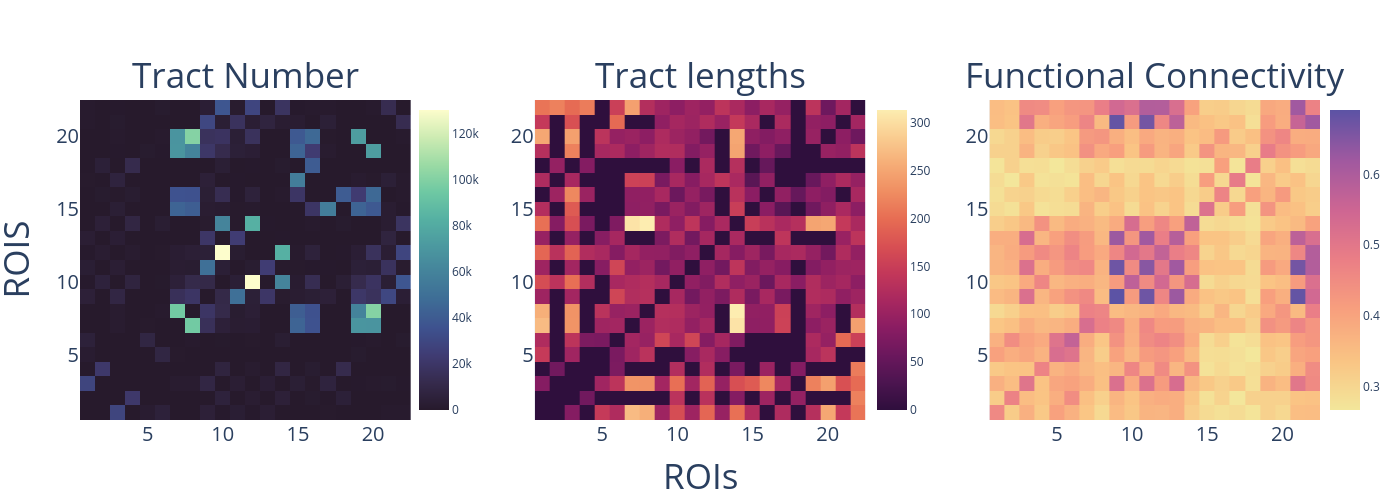
\includegraphics[width=\textwidth]{chapter3/figures/matrices-data.png}
%     \caption{Structural and functional connectivities of subject 04. 
%     From left to right: the number tract matrix, the tract length matrix and the functional connectivity. \textcolor{blue}{To make: same plot with the whole set of subjects, maybe only 5 and the rest in the appendix.}}
%     \label{fig:matrices_data}
% \end{figure}
\begin{figure}[htbp]
    \centering
    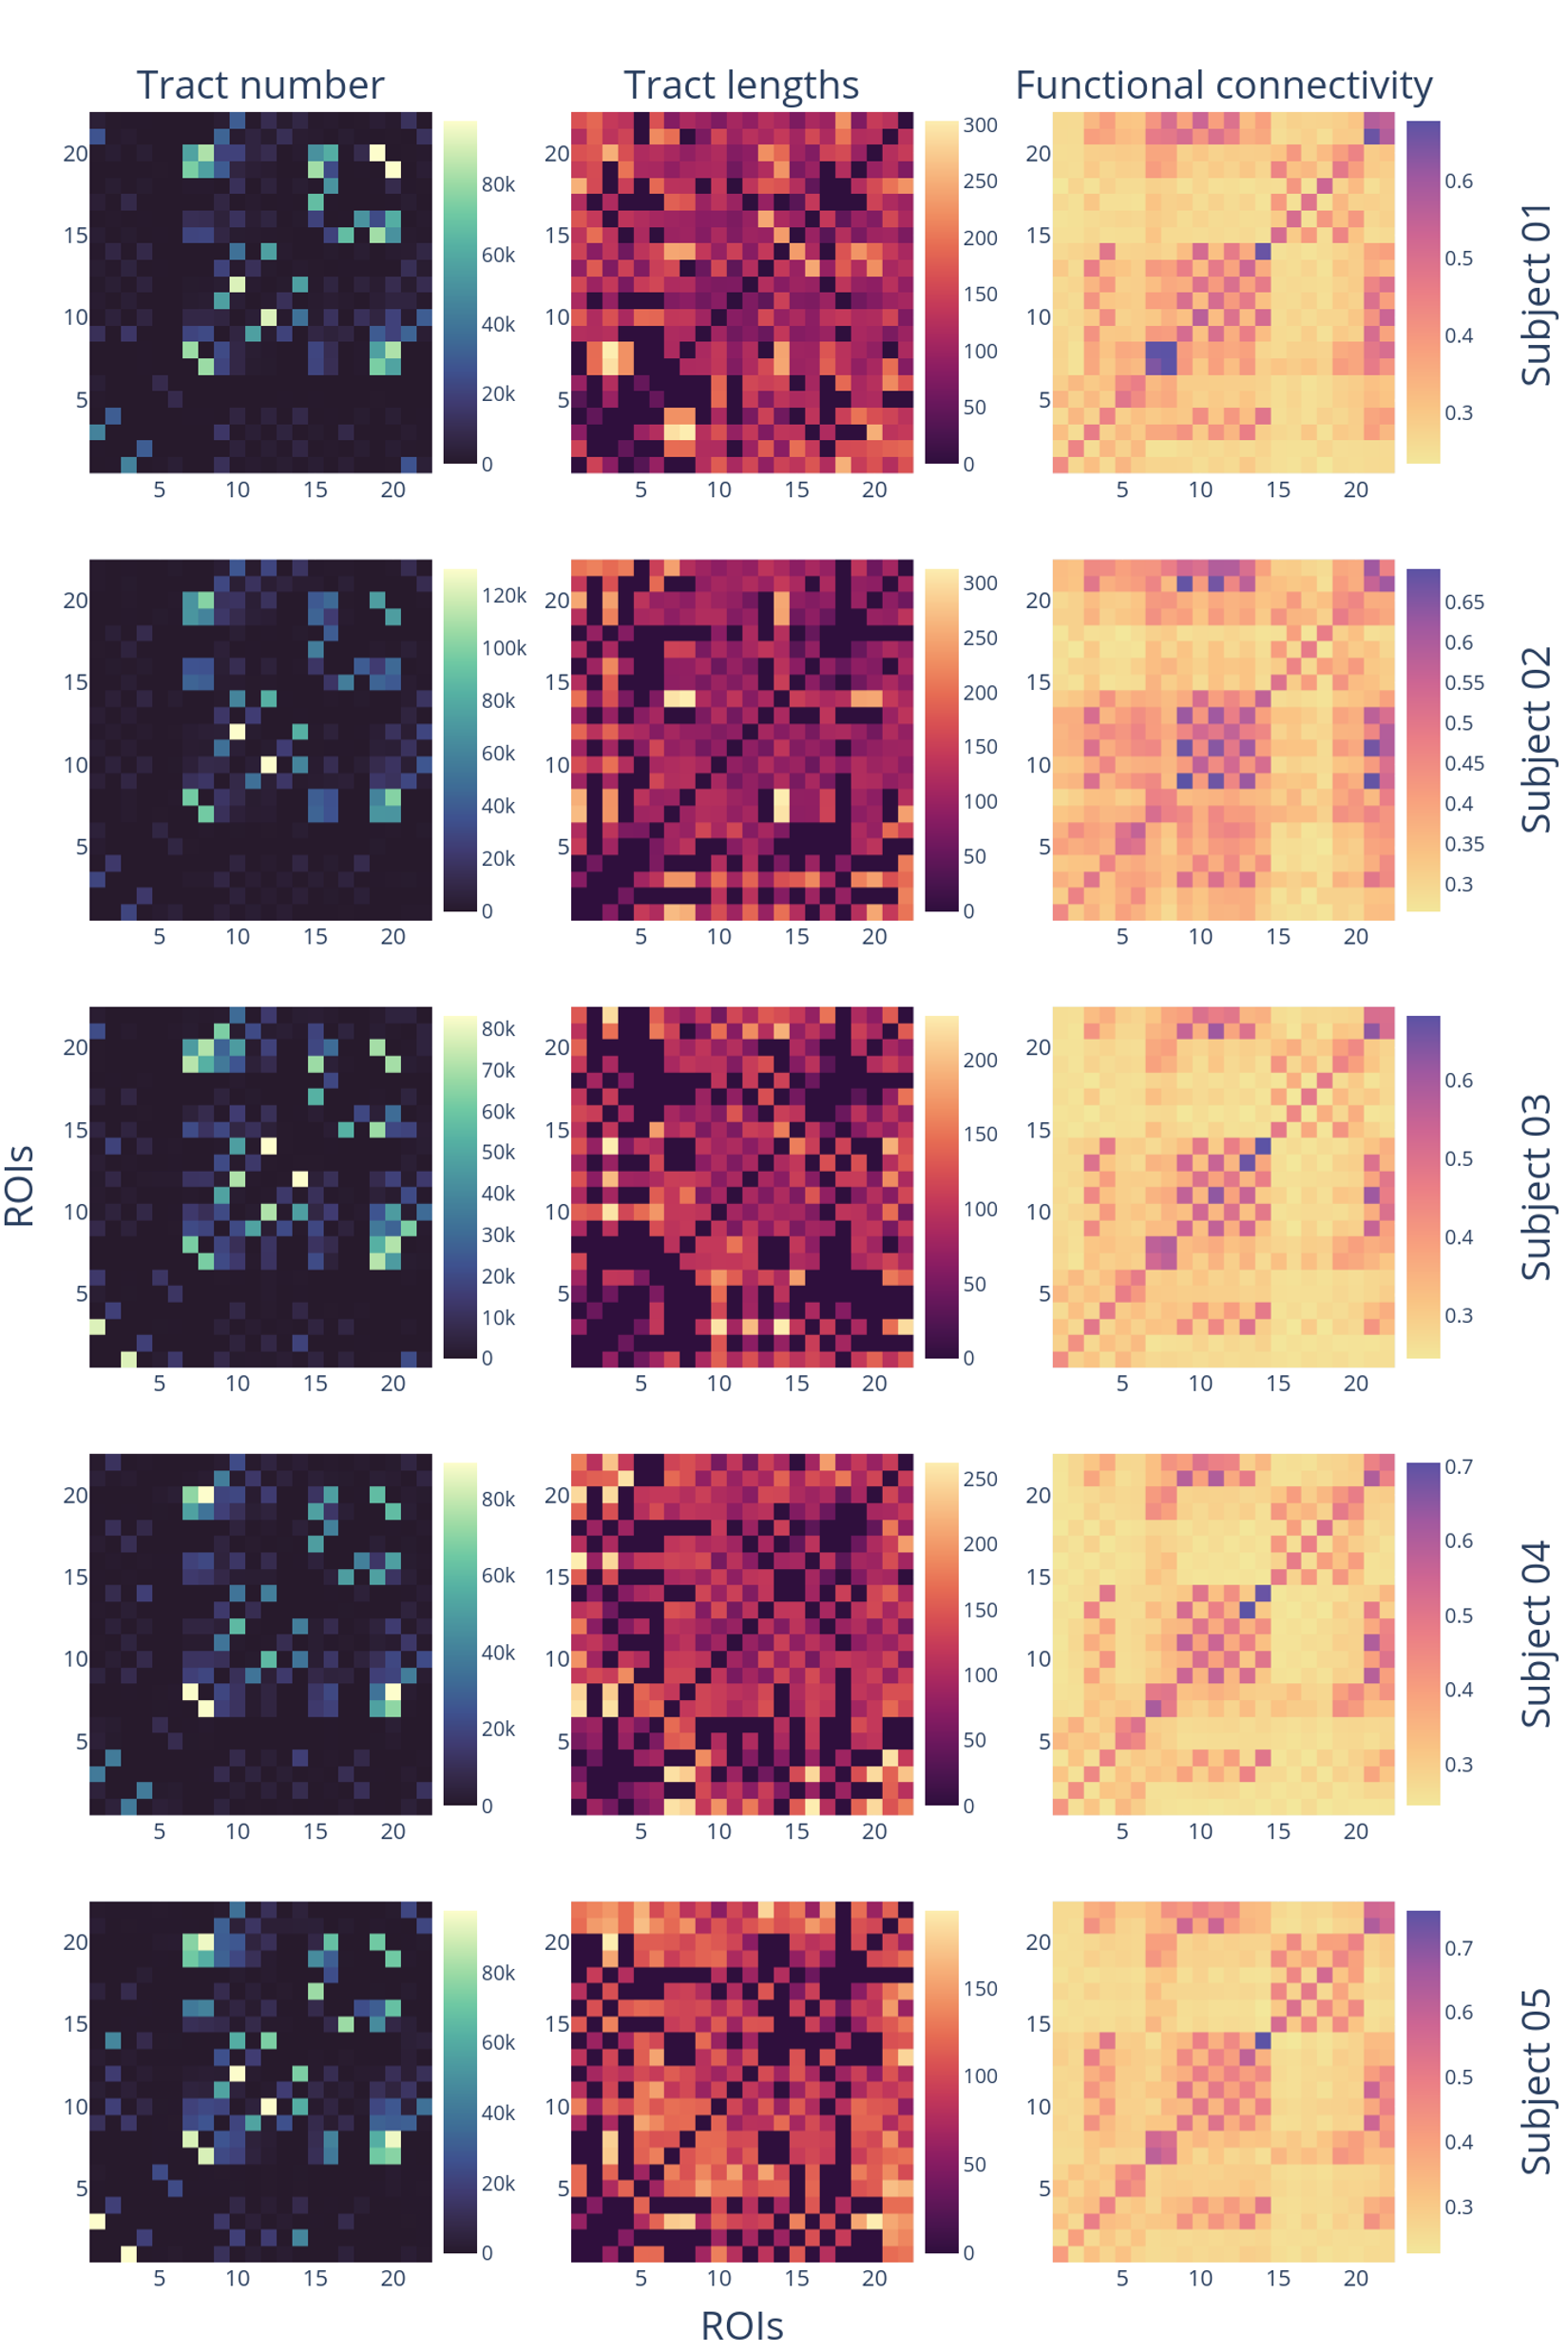
\includegraphics[width=0.90\textwidth]{chapter3/figures/empirical_matrices_0.png}
    \caption{\textbf{Structural and functional connectivity matrices}.
    From left to right: the number tract matrix, the tract length matrix and the functional connectivity of subjects 01 - 05.}
    \label{fig:matrices_data}
\end{figure}
\begin{figure}[htbp]
    \ContinuedFloat % To indicate continuation of the previous table
    \centering
    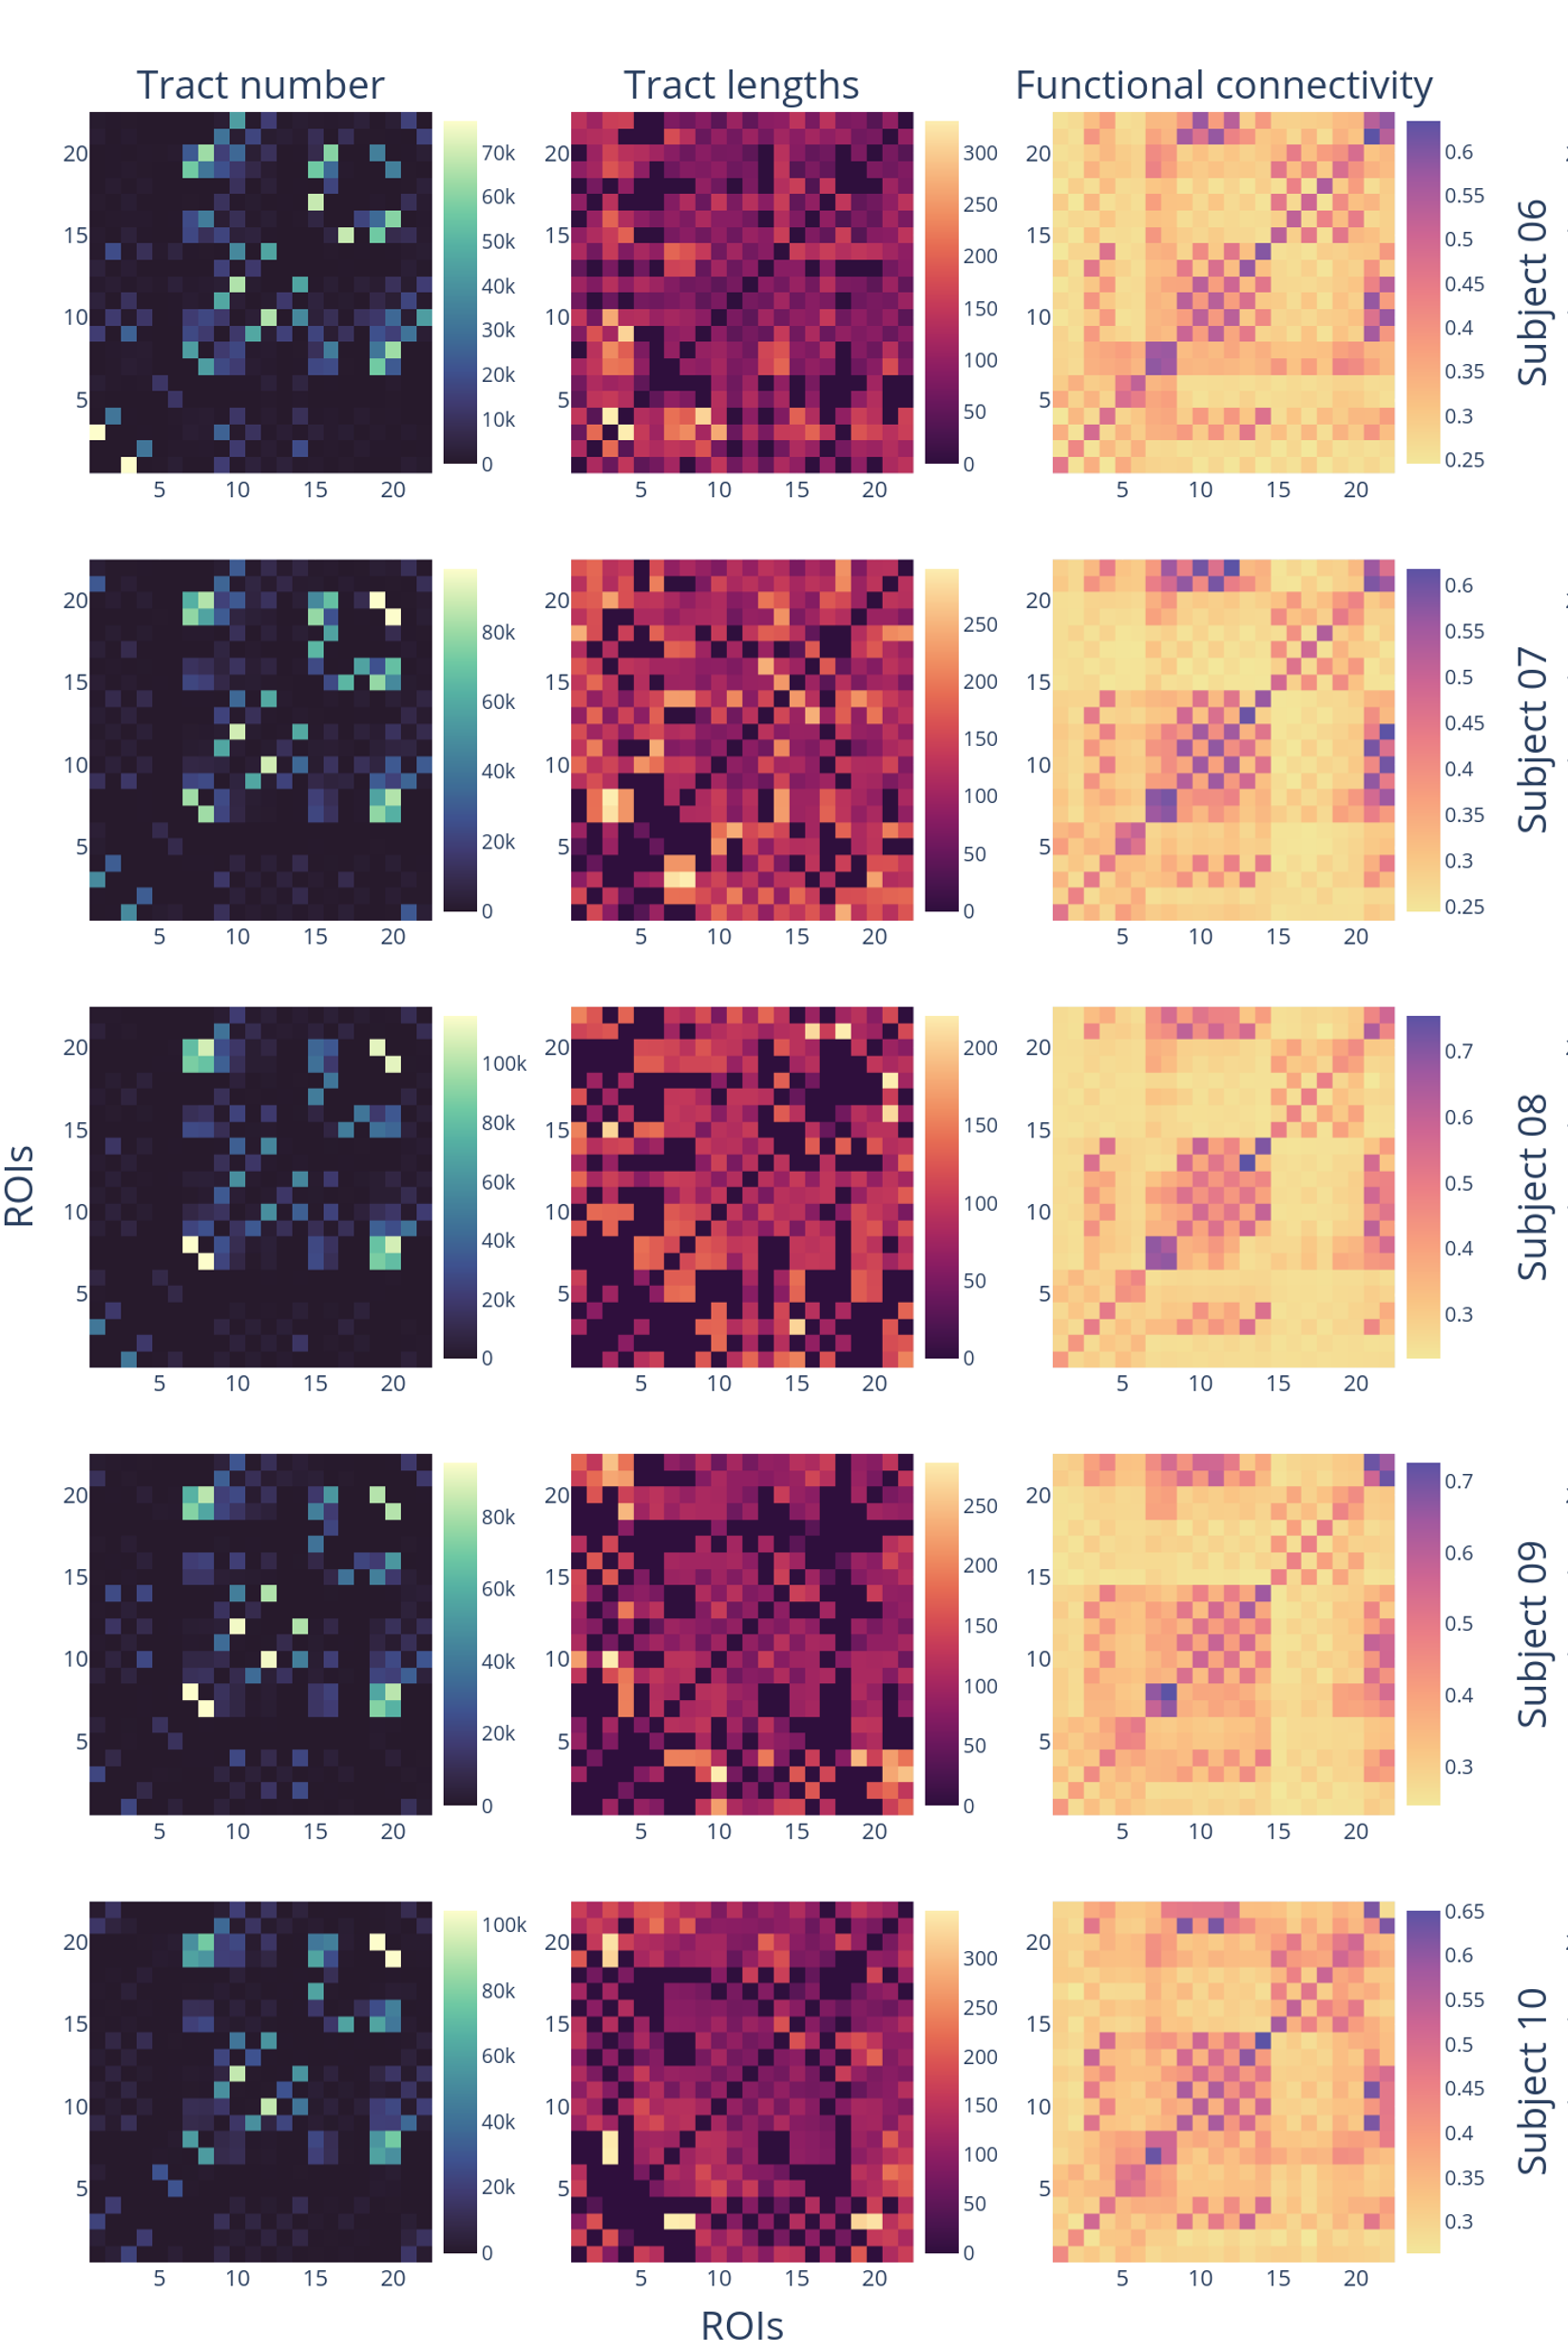
\includegraphics[width=0.9\textwidth]{chapter3/figures/empirical_matrices_1.png}
    \caption{\textbf{Structural and functional connectivity matrices (continuation)}.
    From left to right: the number tract matrix, the tract length matrix and the functional connectivity of subjects 06 - 10.}
    % \label{fig:matrices_data_2}
\end{figure}

\subsection{Phase locking value}
Phase-locking value (PLV) measures the phase synchronization between two narrow-band signals and is the metric used for computing the functional connectivity.
Given a pair of time series $s_1(t)$ and $s_2(t)$ (the LFP signals in our study), that were band-pass filtered to a frequency range of interest (alpha band).
Analytic signals $z_i(t) = A_i(t)e^{j\varphi_i(t)}$ for $i = {1, 2}$ from $s_i(t)$ were obtained using the Hilbert transform \citep{cohen_time-frequency_1995}:
\begin{equation}
    z_i(t) = s_i(t) + j\text{HT}(s_i(t)),
    \label{eq:analytic-signal}
\end{equation}
where HT is the Hilbert transform and is defined as 
\begin{equation}
    \text{HT}(s_i(t)) = \displaystyle\frac{1}{\pi}\displaystyle\int_{-\infty}^{\infty}\displaystyle\frac{s_i(t)}{t-\tau} dt.
    \label{eq:hilbert-transform}
\end{equation}
Then, the relative phase can be computed as:
\begin{equation}
    \Delta\varphi(t) = \arg\Bigg(\displaystyle\frac{z_1(t)z_2^{*}(t)}{|z_1(t)||z_2(t)|} \Bigg).
    \label{eq:phase-diff}
\end{equation}
Finally, the PLV is given by:
\begin{equation}
    PLV = \big|\text{E}\big [ \exp{(j\Delta\varphi_i)} \big] \big|,
    \label{eq:plv}
\end{equation}
\clearpage
where E[$\cdot$] is the expected value.
The PLV is a metric that ranges from 0 to 1, where a value of 0 indicates no phase synchrony between two signals, and a value of 1 indicates that the relative phase between the two signals is identical.

% \subsection{Working point}
% \textcolor{blue}{Esta parte está bien desarrollada y comentada en la parte de resultados, por tanto no se si esto tiene cabida aquí.
% Por un lado, la búsqueda del working point si que es un método como tal, pero hago una comparativa entre el método clásico y lo que he hecho...}

% A commonly used protocol for aligning the model with empirical observations involves determining the optimal coupling factor that maximizes the similarity between experimental functional connectivity (eFC) and the functional connectivity resulting from the simulation (sFC).
% The level of similarity is typically assessed using the Pearson correlation between vectorized upper triangular matrices.
% Therefore, the best fit is achieved when this correlation is maximized \citep{cabral2014exploring,nakagawa_how_2014}.
% However, we incorporated few additional conditions: Firstly, to prevent highly synchronized states at the region level, we excluded unrealistically high mean phase locking value (PLV) values as a criterion for selecting the working point.
% Secondly, to explore alpha frequency bands relevant to our study, we imposed that the different nodes in the network had to oscillates within the alpha range, and more exactly, as close to 10 Hz.
% These simulations were conducted three times, each lasting 25 seconds, with the initial 4 seconds removed to eliminate transients.

\subsection{Current propagation model}
The design and execution of the current propagation model, similar to data acquisition and processing, were carried out by our collaborators at the C3N.

To estimate the electric field generated in the brain, our collaborators employed an Oz-Cz (midline occipital and midline central, respectively) stimulation protocol.
This estimation was performed using the ROAST software \citep{huang2018roast}.
ROAST utilizes MRI-T1 images to segment brain tissues and create a volumetric mesh using the Finite Element Method (FEM).
By solving the underlying Laplace's equation, the software calculates the electric field propagation through the brain under direct current (DC) stimulation \citep{huang2018roast}.
The primary output of the model is an electric field vector for each MRI voxel, illustrated in  Figure \ref{fig:fig1}.
\begin{figure}[htbp]
    \centering
    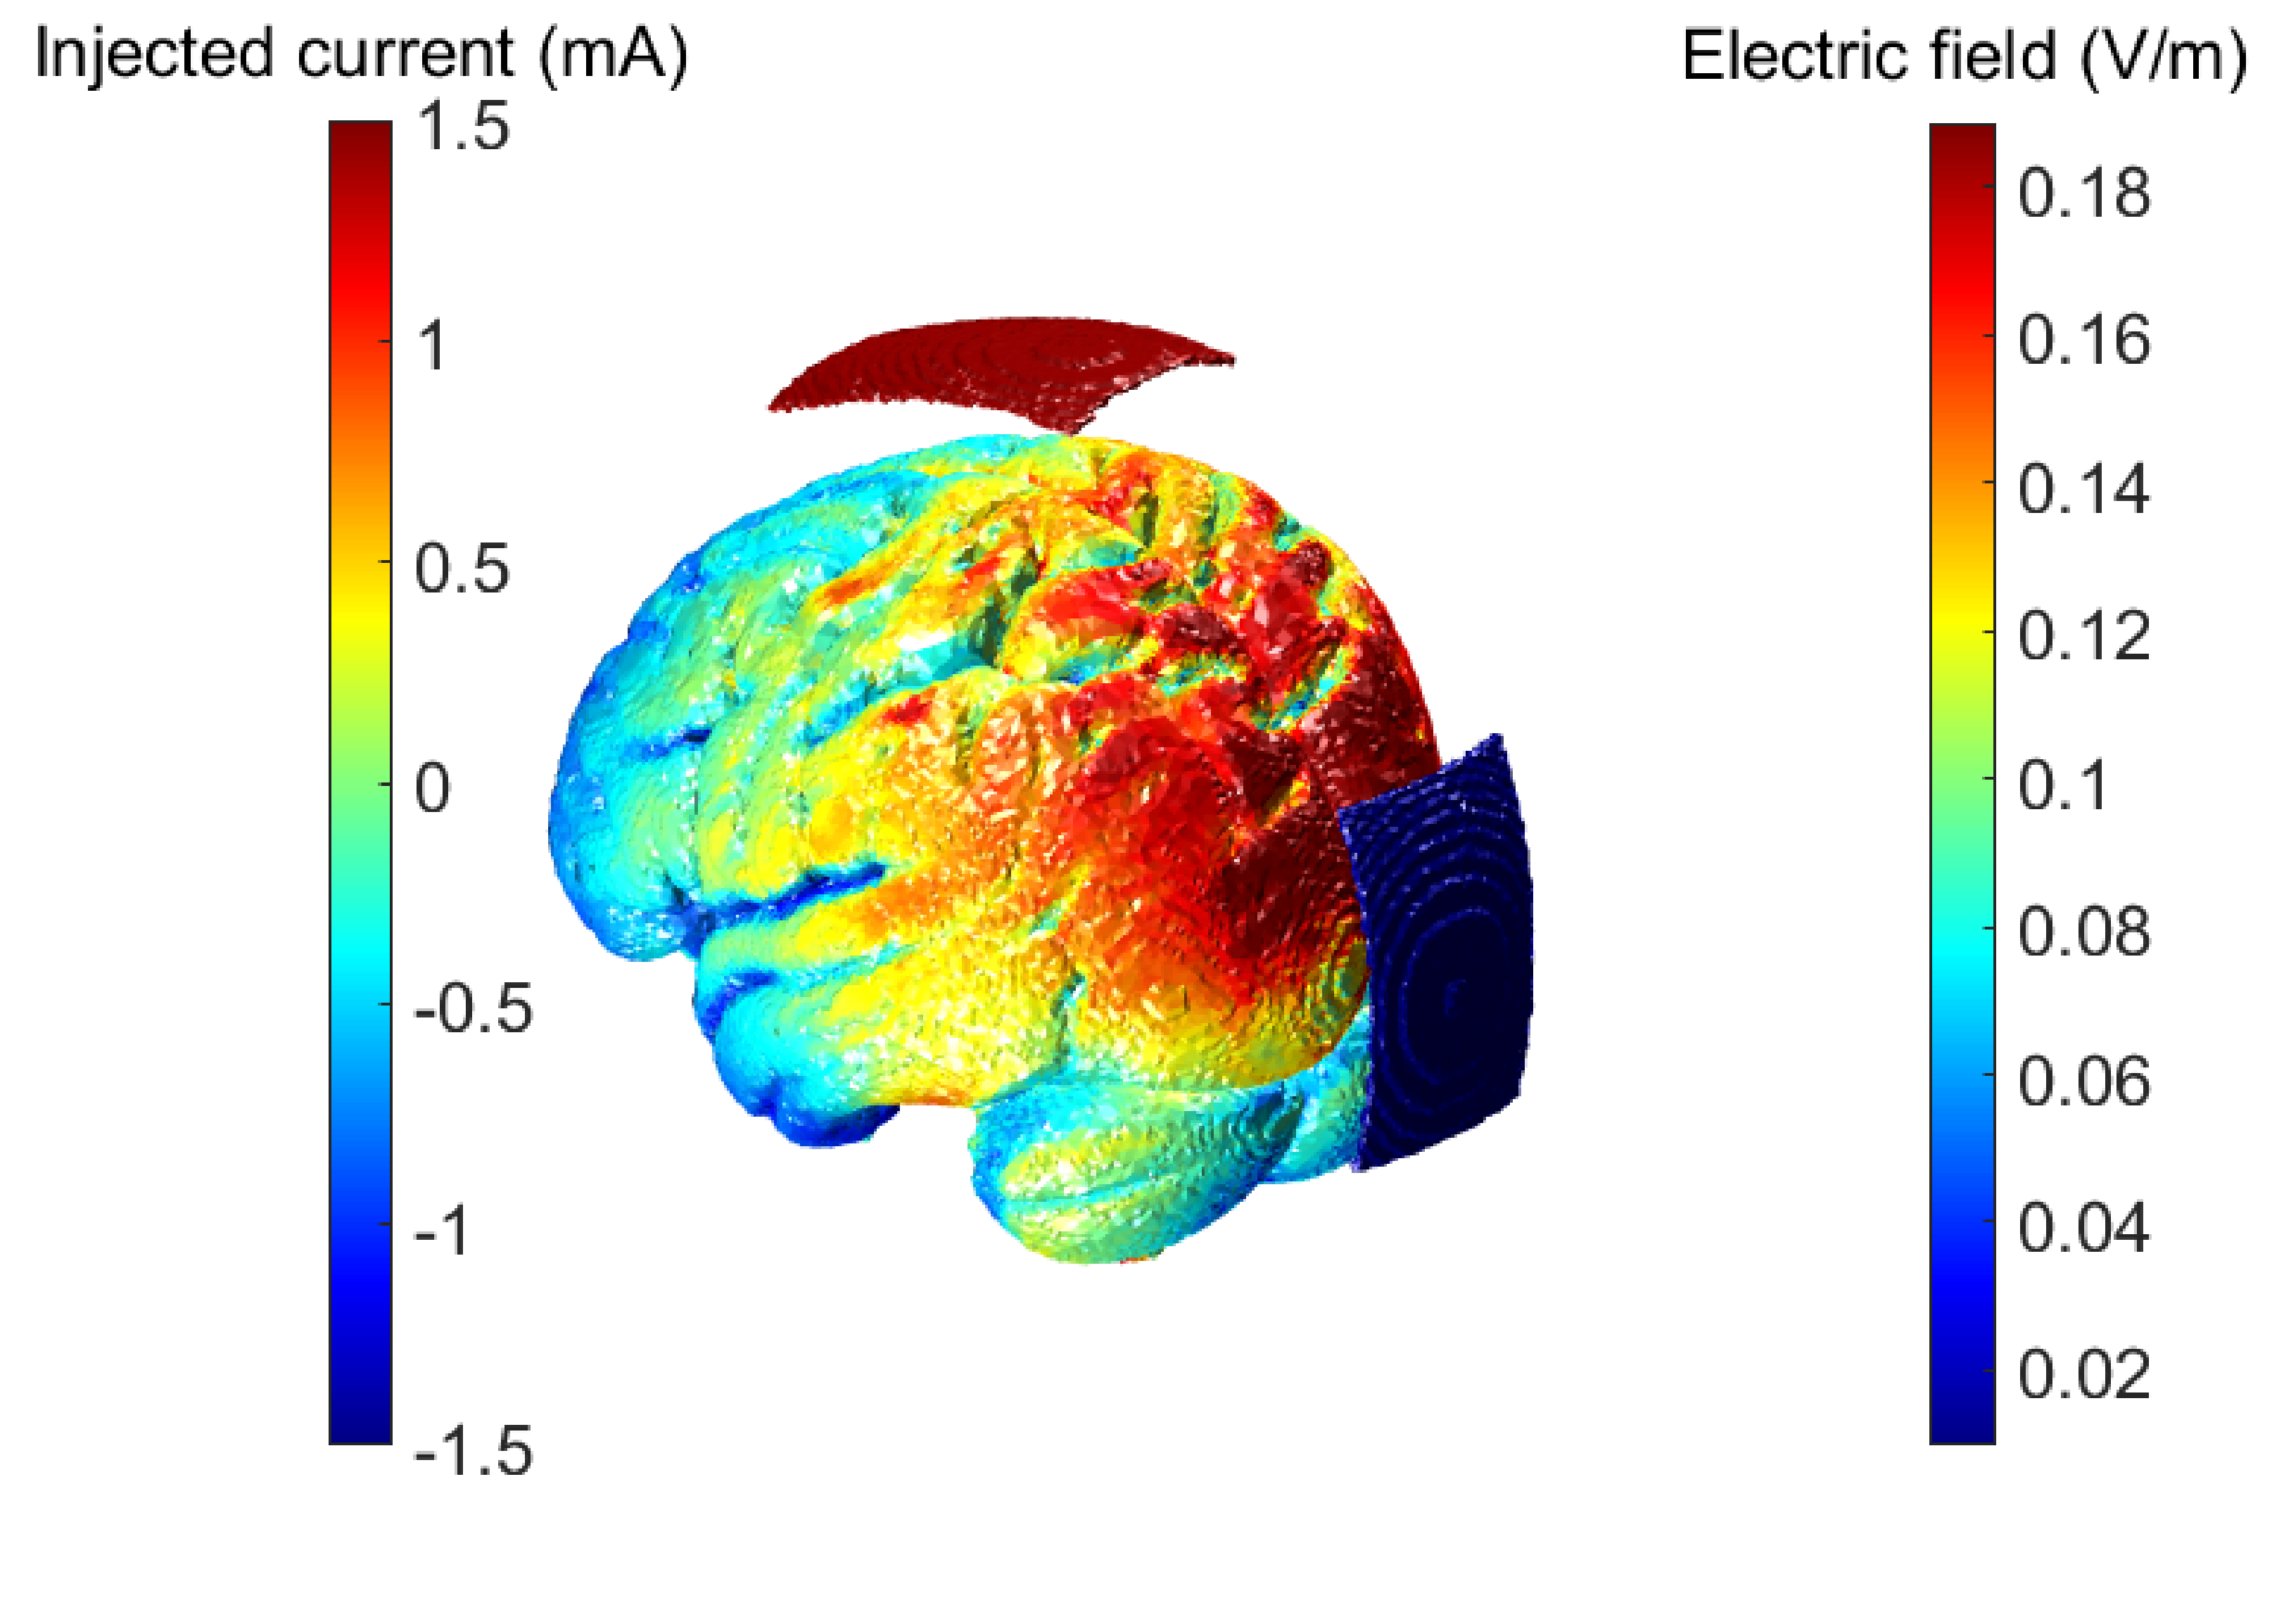
\includegraphics[width=0.75\textwidth]{chapter3/figures/1.png}
     \caption{\textbf{Electric field propagation}.
     Magnitude of the electric field given by ROAST using a Oz-Cz protocol,
     where \textit{pareto-occipital} regions are being stimulated.
     The left side colorbar refers to the injected current at the electrodes, while  
     the right one refers to the resulting magnitude of the electric field for each cortical voxel.
     Original figure from \citep{cabrera-alvarez_understanding_2023}.}
    \label{fig:fig1}
\end{figure}
\clearpage
Additionally, the orientation of the pyramidal cells' body axis was considering by using an isometric triangular mesh of the boundary surface between white and gray matter.
In this way, the values of the normal components of the electric field $E_{t\perp}$ referred to each surface triangle $t$ were computed through the scalar product.
The equation used for calculation is as follows:
\begin{equation}
    E_{t\perp} = \vec{E_t} \cdot \hat{n_t} = |E_t| \cos{\theta_t}.
    \label{eq:perpendicular-components}
\end{equation}
Here, $\hat{n_t}$ represents the unit vector perpendicular to triangle $t$ and points towards the white matter volume.
This approach allows to determine the normal components of the electric field for different surface triangles.
Fields with their normal component aligned with the orthodromic direction (dendritic tuft to axon) will result in positive values, while those aligned with the antidromic direction will result in negative values \citep{bikson2004effects,merlet_oscillatory_2013}.
For each subject, the normal components of the electric fields were grouped for each region $k$ of the  AAL atlas, generating a set of distributions $E_{k\perp}$.
Figure \ref{fig:fig2} shows the produce followed to estimate the normal components of the electric field.

% In Figure \ref{fig:fig5} we show the acumulated distributions of the normal components of all the ten subjects.
To implement the transcranial alternating current stimulation (tACS) in the simulations, we utilized the region-specific distributions to generate a set of sinusoidal currents.
Therefore, these currents had heterogeneous amplitudes with a fixed frequency.
The current input for the neuron $i$ belonging to node $k$ is given by the equation:
\begin{equation}
    I_{ext,i}^k(t) = \Lambda A_i^k  \sin{(2 \pi f t)},
    \label{eq:tacs}
\end{equation}
where $A_i^k$ is a random value generated by the distribution $\{E_{k\perp}\}$.
The effective amplitude of the stimulation is determine by the product between that value and the global stimulation intensity denoted by $\Lambda$.
The units of ${E_{k\perp}}$ are V/m, hence the units of $\Lambda$ are $pS\cdot m$ in order to match the current units to pA.
\begin{figure}[!htb]
\centering
\includegraphics[width=\textwidth]{chapter3/figures/2.png}
 \caption{\textbf{Estimation of the electric field normal components}.
 The electric $E_{t\perp}$ field normal component on triangle $t$ of the white matter surface computed as the dot product between the electric field $\vec{E_t}$ in this point (computed by Roast), and the normal vector $\hat{n_t}$ to the surface $t$ (the triangular mesh).
 Note that $\hat{n_t}$ represents the direction of the cortical columns subtended to this area of cortex.
 Red colour indicates a sagital section of the gray matter, where blue colour indicates its inner and outer surfaces.
 ROI-specific distributions of the normal components of $E_{k\perp}$ are used for the stimulation of spiking populations.
 Original figure from \citep{cabrera-alvarez_understanding_2023}.}
\label{fig:fig2}
\end{figure}

\subsubsection{Distributions of normal components of electric field}
tACS currents primarily affect pyramidal cells and that their relative mismatch between the electric field direction and cell body axis influences the stimulation efficacy.
Evaluation of the electric field direction with respect to the normal vectors of the triangulated surface between white and grey matter revealed two types of distributions: unimodal and bimodal distributions, varying based on the position and shape of different brain regions.
Figure \ref{fig:fig5} illustrates the combined distributions of the normal components across all ten subjects

The distributions exhibited positive (oriented towards white matter) and negative values of $E_{t\perp}$, perpendicular to the direction of the electric field, indicating the presence of pyramidal cells aligned parallel or antiparallel to the electric field.
Regions aligned with the anterior-posterior axis, such as the cingulate cortex, insula, and middle frontal gyrus,
\begin{figure}[!htb]
    \centering
    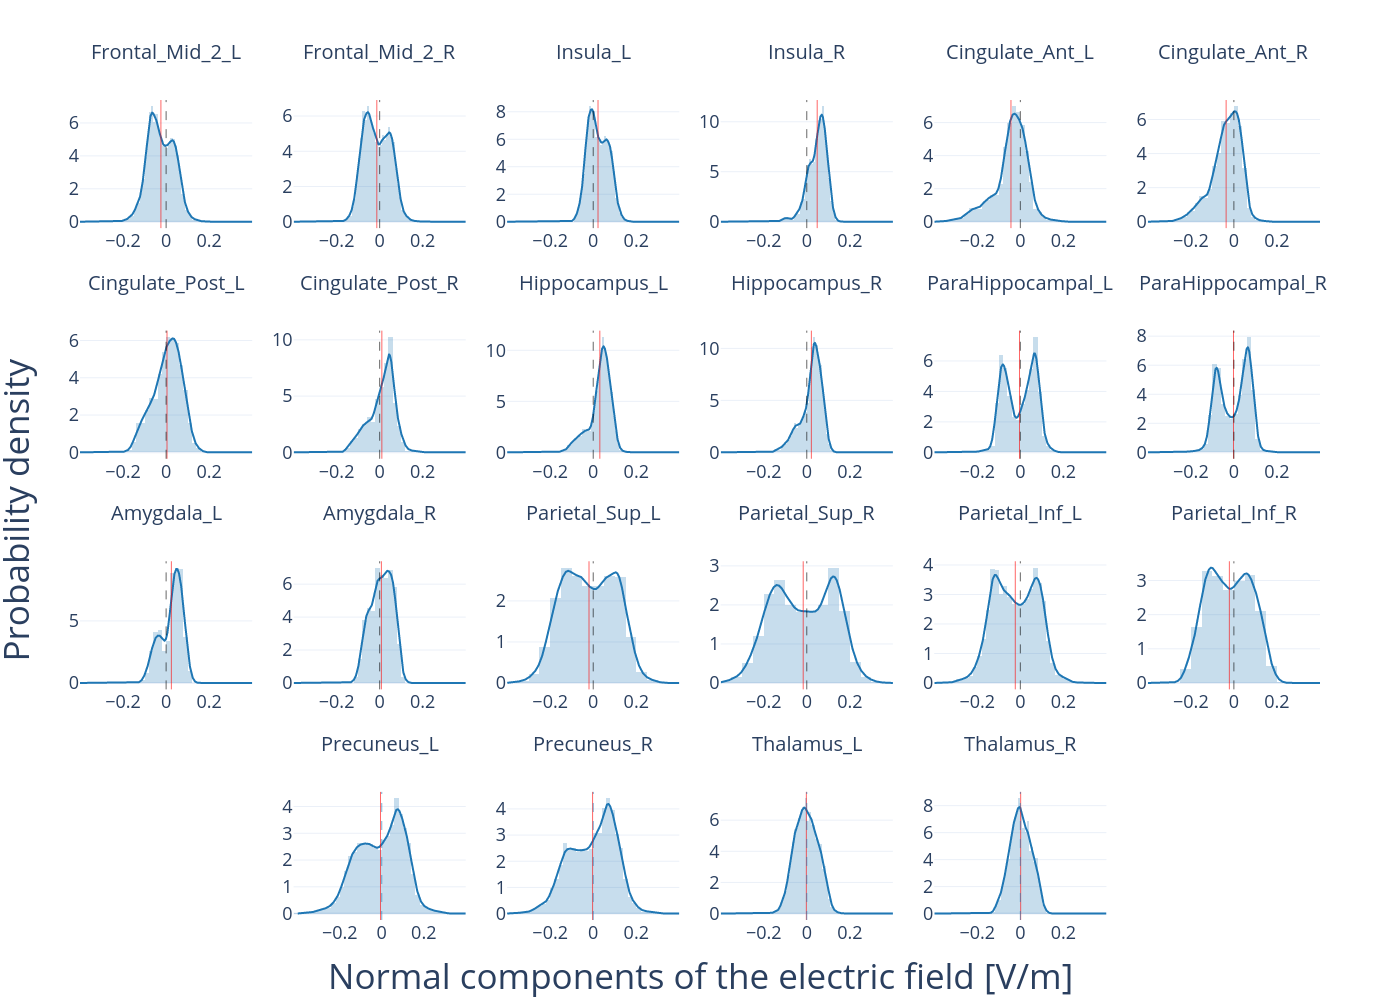
\includegraphics[width=\textwidth]
    {chapter3/figures/5.png}
    \caption{\textbf{Electric field normal component distributions} $\mathbf{E_{k\perp}}$.
    Each histogram shows the accumulated distribution (across the ten subjects) of normal components to the white matter surface of the electric field generated by the Oz-Cz stimulation protocol over the regions of the cingulum bundle.
    Vertical red line represents the mean of the distribution.}
    \label{fig:fig5}
\end{figure}
displayed unimodal distributions with slight skewness, resulting in an increased absolute value of the mean.
The level of gyrification was found to be related to the strength of bimodality observed.
For example, the cingulate cortex exhibited less bimodality compared to the more intricate middle frontal gyrus. Interestingly, these regions showed a consistent bias towards the same value in both hemispheres. 

In contrast, posterior regions such as the parietal cortices and the precuneus, which have a higher degree of gyrification, exhibited bimodal distributions.
These regions displayed highly symmetric distributions around zero, with two distinct peaks.
This suggests that the gyri in these regions are primarily oriented perpendicular to the electric field.
Therefore, stimulating these regions with the Oz-Cz protocol could lead to hyperpolarization of certain cells while depolarizing others.
However, the precise interactions of these regions within a network and their effects on pyramidal cells in the gyrus are still not fully understood.

\subsection{Implementation of tACS in our model}
First, simulations were conducted on isolated nodes to examine the impact of various hypothetical shapes on the distribution of normal components in the underlying neural activity: symmetric bimodal, symmetric shifted bimodal and gaussian.
To evaluate the effects of stimulation, by varying the stimulation frequency and the amplitude, we analyzed the power spectral density (PSD) of the simulated population. 
This analysis provided information on the frequency peak of the nodes as well as the power values at both the peak and stimulation frequency.

Subsequently, we implement the stimulation into the resting-state network model by varying the stimulation  $\Lambda$ and frequency equal to the IAF of each personalized model.
%\textcolor{blue}{These simulations specifically focused on cingulum bundle networks and involved ten subjects from the computational dataset.}
Both types of simulations were repeated ten times, with each simulation lasting for 50 seconds.
The initial 4 seconds of each simulation were excluded to account for potential transients.

% \subsubsection{Statistics}
% \textcolor{blue}{Dudoso de incluir esto aqui. De ponerlo lo pondría en los resultados y ahi mismo se explica que el análisis hecho.
% Esta parte no está cambiada en nada respecto al paper}
% We checked for statistically significant differences between the baseline simulations and the fitted using Wilcoxon’s ranked comparisons \citep{wilcoxon1992individual} due to the small sample size, and correcting significance with a step-down method using Bonferroni adjustments \citep{holm1979simple}.

% To evaluate the impact of different variables on the increase of alpha power, we performed a stepwise multiple linear regression.
% We considered 7 candidate variables per region:
% the electric field modelled through the distributions of normal components; the squared value of the mean (as the effect is expected to be equivalent for negative and positive values and to linearize the data), the \textit{skewness}, the \textit{kurtosis},
% the number of \textit{modes}; the structural connectivity, with the logarithm of the nodes’ \textit{connectivity strength} to linearize the exponential shape observed in the structural connectivity data, the network function before stimulation, using the average PLV value, and the frequency difference between the stimulation and the node’s baseline oscillation. 

% Two variables were transformed to get a better fit for the data.
% We used the square of the mean of the normal components of the electric field with the purpose of obtaining.
% Additionally, we used the base 2 logarithm of the node strength to get a better fit to the structural connectivity data.

% The values of these variables were normalized in order to get a meaningful comparison of the resulting coefficients.
% Due to the violation of residuals’ normality, we used an iteratively reweighted least squares algorithm as a robust version of the multiple linear regression. The weighted function for residuals was a Huber’s T


\end{document}